% Előzmények (irodalomkutatás, hasonló alkotások), az ezekből levonható következtetések

% előző scriptek
% hivatalos programok is csak griden
% hol használnak még ilyet nyomtatáson kívül (üveg)
% ládapakolás, np nehéz
% extra megkötés, vágóasztallal vágás
% talált irodalom
% felhasznált pszeudokód? idk
% egyéb algoritmusok a strip packingen kívül

\chapter{Előzmények és irodalomkutatás}

\section{Hivatalos szoftverek}

A Canon imagePROGRAF PRO-4600 plotterhez több különféle nyomtatási segédprogramot is járt. A használatukra való áttérés meghiúsult, mert alapvető funckiók hiányoztak belőlük. A legtöbb program csak kézzel való elrendezést tett lehetővé, a mi esetünkben ez viszont egy visszalépést jelentett volna a szkripttel szemben.

\section{A Photoshop szkriptről}

A szkript által használt algoritmus felettébb egyszerű. A dokumentumo\footnote{A dokumentum az elkészült kép, a program kimenete, melyen a bemeneti forrásfájljaink szerepelnek.} egy rács mentén cellákra kerül felosztásra, ahol minden cella mérete a kinyomtatni kívánt kép méretének felel meg.
Nem mindegy, hogy a cellák fekvő vagy álló tájolással vannak elhelyezve a dokumentumon, ugyanis ez különböző mennyiségű felesleget eredményezhet.

\begin{figure}[!h]
    \centering
    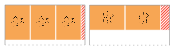
\includegraphics{figures/wastecalc.pdf}
    \caption{Soronként keletkező felesleg eltérő tájolások mellett}
    \label{fig:wastecalc}
\end{figure}

Az orientáció kiszámításához meg kell vizsgálni mindkét esetet egy teljesen kitöltött sorra. Legyen a tekercs szélessége $W$, a keletkező felesleg pedig $A$. Vegyünk egy képet, ahol a kép szélessége $w$, magassága $h$, orientációja $o$. Ekkor a keletkező felesleg

$$m_1 = \bigg\lfloor \cfrac{W}{w} \bigg\rfloor, \qquad A_1 = (W - m_1 * w) * h,$$

\noindent illetve ellentétes orientáció esetén

$$m_2 = \bigg\lfloor \cfrac{W}{h} \bigg\rfloor, \qquad A_2 = (W - m_2 * h) * w.$$


A kevesebb felesleget eredényező eset határozza meg az orientációt. Az orientáció alapján kiszámolható a rács oszlopainak száma, $m$. Ez $n$ kinyomtatni kívánt kép esetén $k$ sort eredményez, ahol

$$k = \bigg\lceil \cfrac{n}{m} \bigg\rceil.$$

\noindent Amennyiben

$$ n \mod m \neq 0,$$

\noindent úgy ez az eljárás üres cellákhoz, azaz papírfelesleghez fog vezetni. 
Emiatt született meg az opció a mennyiség korrigálására, mely megnöveli $n$-t úgy, hogy a korrigálás előtti esetleges üres cellákba is kerüljenek képek:

$$n' = k * m.$$

\begin{figure}[!h]
    \centering
    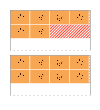
\includegraphics{figures/correct_quantity.pdf}
    \caption{A mennyiség korrigálás}
    \label{fig:correct_quantity}
\end{figure}

Ez a megoldás sajnos nem tökéletes. Ha az utolsó sorunk cellái nincsenek teljesen kitöltve, akkor abban a sorban nem biztos, hogy $o$ orientáció valóban kevesebb felesleggel fog járni (\ref{fig:lastrow}).

\begin{figure}[!h]
    \includegraphics[width=\textwidth]{figures/lastrow.png}
    \caption{Az utolsó sor különböző orientációkban és hatása.}
    \label{fig:lastrow}
\end{figure}

Ilyen esetek miatt az utolsó sort a többitől külön kell kezelni, és figyelembe kell venni a fennmaradó elemek számát. Ekkor az utolsó sor oszlopainak száma

$$m' = n - (k - 1) * m,$$

\noindent a keletkező feleslegek pedig


$$A_1 = (W - m' * w) * h,$$
$$A_2 = (W - m' * h) * w,$$

\noindent melyekből a kisebbik határozza meg az orientációt. Ebben az esetben is releváns lehet az elemek számának korrigálása, ilyenkor

$$n' = (k - 1) * m + m'.$$


\section{Különböző méretű képek elrendezése}

A különböző méretű dobozok fix területre történő elhelyezése a ládapakolási problémára vezethető vissza. A prezentált probléma egy speciális esete ennek. A tekercs szélessége fix, a magassága viszont tetszőleges, de minimalizálni szeretnénk. Az eredménynek vágóasztallal vághatónak kell lennie.

\subsection{Guillotine vágás}

A guillotine vágás egy olyan folyamat, ahol egy nagyobb lemezt vágnak fel előre megadott, kisebb téglalapokra, guillotine vágásokkal. A guillotine vágások, más néven széltől-szélig vágások egyik oldaltól a másik oldalig tartó egyenes vágások, melyek a téglalapot két részre osztják fel. 
Ezt az eljárást elsősorban üveg, acél, fa illetve kartonpapír lapok felvágásakor alkalmazzák. Több különböző szempont alapján is lehet megpróbálni optimalizálni a probléma megoldását, például maximalizálni a kapott elemek területét, értékét vagy számát illetve minimalizálni a szükséges vágások számát vagy a keletkező felseleget (\cite{guillotine-cutting-wiki} alapján).

A guillotine vágás esetén a lemezek mérete előre meg van adva, és a kisebb téglalapok mennyisége nincsen megkötve. A prezentált probléma nagyban hasonlít a guillotine vágásra, leszámítva, hogy a képek mennyisége fix, és csak a tekercs szélessége adott. 

\begin{figure}[!h]
    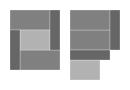
\includegraphics[width=\textwidth]{figures/guillotine_cutting.pdf}
    \caption{Egy nem guillotine vágás és egy guillotine vágás.}
    \label{fig:guillotine}
\end{figure}

\subsection{Tekercsre pakolás probléma}

A tekercsre pakolás probléma egy két dimenziós geometriai minimalizálási probléma. Adott egy tekercs fix szélességgel és tetszőleges magassággal, valamint a tekercsre helyezendő téglalapok. Meghatározandó egy elrendezés, mely átfedés nélkül helyezi el a téglalapokat a tekercsre, minimalizálva a felhasznált tekercsrész magasságát. Legtöbbet a textil- és papírtekercsek feldolgozásával foglalkozó területeken találkozhatunk ilyen megoldásokkal.

Sajnos a tekercsre pakolási probléma erősen NP-nehéz, mert magában tartalmazza a ládapakolási problémát fix magasságú elemekkel (\cite{strip-packing-wiki} alapján).

A feladat tehát visszavezethető a tekercsre pakolás és a guillotine vágás keveréke, egy tekercsre kell guillotine-nal vágható elrendezésben pakolnunk az elemeinket. Szerencsére ez már egy ismert speciális esete a tekercsre pakolásnak, és több különféle algoritmus is létezik már rá.

\section{A választott algoritmusok}

Egyetlen méret nyomtatása esetén a régi szkript kapcsán ismertetett rácsra helyezés javított változata már egy optimális megoldás, és adott a lehetőség a mennyiséget korrigálására az esetleges ki nem töltött cellák alapján. 

Különböző méretű képek esetén a probléma erősen NP-nehéz voltából adódóan a keresett megoldás nem kellett, hogy optimális legyen, mert fontos szempont volt a program futásának ideje, és mert az egyszerre több különböző méretben való nyomtatás egy viszonylag ritka esetnek minősül.  

A \cite{ph} cikkben többek közt az ismertett problémára mutatnak be egy heurisztikus megoldást. Az algoritmus heurisztikus voltából adódóan nem ad mindig optimális megolást, komplexitása azonban csupán $O(n^2)$. A megoldás egy rekurzív megközelítést alkalmaz, ami elősegíti, hogy az eredmény biztosan vágóasztallal vágható legyen. 
A cikkben bemutatott koncepció egyszerű: az elemeket egy téglalapra kell helyezni, minden lehelyezett elem további téglalapokat határoz meg. Egy elem elhelyezésénél öt különböző eset állhat fenn.

\begin{figure}[!h]
    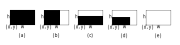
\includegraphics[width=\textwidth]{figures/priority.pdf}
    \caption{A lehetséges esetek egy elem elehelyezésekor. A fekete téglalapok az elemet jelölik.}
    \label{fig:placements}
\end{figure}

Az \href{fig:placements}{(a)} eset a legkedvezőbb, ebben az esetben a rendelkezésre álló helyet az elem teljesen kitölti. A \href{fig:placements}{(b)} és \href{fig:placements}{(c)} esetek kedvezőbbek, mint \href{fig:placements}{(d)}, mert ekkor az üresen maradt hely egyetlen téglalapot eredményez. Az \href{fig:placements}{(e)} esetben egyetlen elemet sem lehet a téglalapra helyezni, a terület ekkor felesleggé válik.

Az elemek elhelyezése előtt minden elemet a rövidebbik élére állítva valamilyen heurisztika alapján sorba kell őket rendezni (pl. magasság szerint csökkenő sorrendbe). Az ábra (\ref{fig:placements}) alapján \href{fig:placements}{(a)}-\href{fig:placements}{(e)} esetekhez rendre prioritások rendelhetők, ahol az \href{fig:placements}{(a)} eset prioritása a legnagyobb. 
Ennek tudatában meghatározható minden hátralevő elem prioritása, mind álló, mind fekvő helyzetben. Legyen a lehelyezendő elem bármelyik orientációban vett legmagasabb prioritású elem, aszerint forgatva, amelyik esetben magasabb a prioritása. 
Ha két elemnek megegyezik a prioritása, a sorba rendezésbeli helyük alapján a sorban előrébb lévő elemet kell figyelembe venni, azon belül pedig a fekvő tájolású elemnek van magasabb prioritása.

Az így kapott elem az adott orientációban elhelyezésre kerül a téglalapon. 
A \href{fig:placements}{(d)} esetben nem mindegy, hogy a lehelyezett elem hogyan osztja tovább a téglalapot. 
A hátralevő elemek közül meg kell határozni a legrövidebb előforduló oldal hosszát, legyen ez $s_\text{min}$. 

\begin{figure}[!h]
    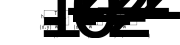
\includegraphics[width=\textwidth]{figures/partitioning.pdf}
    \caption{A téglalap lehetséges felosztása}
    \label{fig:partitioning}
\end{figure}

Az ábra (\ref{fig:partitioning}) alapján amennyiben $w - s_1 < s_\text{min}$, úgy \href{fig:partitioning}{(d\textsubscript{1})} szerint lehet csak felosztani a területet, mert ekkor T\textsubscript{2} téglalapra egyik esetben sem fér el semelyik elem sem, azaz ez a rész felesleggé válna.
Hasonlóképpen ha $h - s_2 < s_\text{min}$, akkor \href{fig:partitioning}{(d\textsubscript{2})} szerint lehet csak felosztani a területet, és T\textsubscript{1} válik felesleggé. 
Amennyiben egyik feltétel sem teljesül, úgy a téglalap kétféleképpen is felosztható. A felosztást $s_1 < s_\text{min}$ feltétel határozza meg: ha teljesül, akkor \href{fig:partitioning}{(d\textsubscript{1})} eset kerül kiválasztásra, mert ellenkező esetben T\textsubscript{1} felesleggé válna.

A keletkező üres téglalapokra újból meghatározásra kerülnek a hátralevő elemek prioritásai és rekurzívan folytatódik a pakolás, amíg minden elem elhelyezésre nem került, vagy elfogytak a téglalapok, amikre elemet lehetne helyezni.

Adott elemekre más-más sorba rendezési heurisztikák más-más elrendezéseket eredményeznek, ezért nem mindegy, hogy hogyan kerül megválasztásra a sorrend. Az elemhalmaztól nagyban függ, hogy éppen milyen szempont alapján érdemes az elemeket sorba rendezni, de ezt nehéz előre meghatározni. Érdemes az algoritmust több különböző sorba rendezés szerint futtatni, és az eredmények közül a legkedvezőbbet választani. Ilyen rendezések lehetnek például magasság, terület, kerület, átló szerinti csökkenő sorrendek.

% TODO egyéb heurisztikák